\documentclass[tikz]{webquiz}
\title{A tikz example}
\begin{document}
  \begin{question}     % a quiz question
     What number is represented by the dot on the following number line?
     \begin{center}
       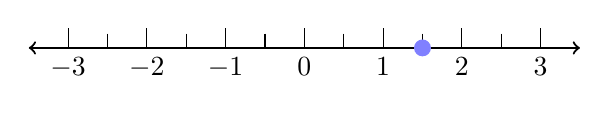
\begin{tikzpicture}
          \foreach \x in {-3,...,3} { \draw(\x,0.25) --(\x,0)node[below]{$\x$}; }
          \foreach \x in {-2.5,...,2.5} { \draw(\x,0.18) --(\x,0); }
          \draw[thick,<->](-3.5,0)--(3.5,0);
          \filldraw[blue!50!white](1.5,0) circle (1mm);
       \end{tikzpicture}
     \end{center}
     \answer{1.5} % inserts an answer box and specifies the answer as 1.5
     \whenRight Correct!
     \whenWrong Incorrect!
  \end{question}
\end{document}
